\vspace{-0.2cm}
\section{Impact of Distributional Shift}
\label{sec:sampling_distributions}
\vspace{-0.2cm}

%As alluded to in Section~\ref{sec:analysis_nonstationarity}, the choice of sampling distribution $\mu$ is an important design decision can have a large impact on performance. Indeed, it is not immediately clear which distribution is ideal for Q-learning. In this section, we hope to shed some light on this issue.

%\subsection{Technical Background}
% Off-policy data has been cited as one of the ``deadly triads'' for Q-learning~\citep{suttonrlbook}, which has potential to cause instabilities in learning. On-policy distributions~\citep{Tsitsiklis1997} and fixed behavior distributions~\citep{Sutton09a,Maei2010} have often been targeted for theoretical convergence analysis, and many works use importance sampling to correct for off-policyness~\citep{precup2001offpol, munos2016safe}
% However, to our knowledge, there is relatively little guidance which compares how different weighting distributions compare in terms of convergence rate and final solutions.

% Off-policy RL methods applied to the offline RL problem would typically attempt to learn an optimal policy, even though the static dataset may not be generated from an optimal policy. As a result, one issue to emerge is that of \emph{distributional shift}: while these methods can only train a model of the value-function and the policy using state-action tuples from the data, these models  will need to make correct predictions on states and actions sampled from a different distribution encountered upon deployment. In general, models trained via machine learning are not robust when the distribution of inputs changes, indicating that distributional shift can be challenge for off-policy RL methods. Is distributional shift a challenge in offline RL?   

Off-policy RL methods applied to the offline RL problem would typically attempt to learn an optimal policy, even though the static dataset may not be generated from an optimal policy. As a result, one issue that emerges is that of \emph{distributional shift}: while these methods train a model of the value-function and the policy only using state-action tuples from the data, upon deployment, these models will need to make correct predictions on states and actions sampled from a different distribution of the learned policy. In general, models trained via machine learning are not robust when the distribution of inputs changes, indicating that distributional shift can be a challenge for off-policy RL methods. Is distributional shift a challenge in offline RL?

Indeed, theoretically, the effects of distributional shift have been quantified using the notion of a concentrability coefficient~\citep{munos2005erroravi}, a constant typically $\gg 1$, which provides a worst-case error bound on the performance of an off-policy RL method due to distributional shift. To evaluate if this challenge persists empirically as well, we will analyze Q-learning methods for various choices of data distributions in this section.

A crucial design decision we must make is to consider setups that do not confound distributional shift with access to limited data. Therefore, for our study, we provide the underlying algorithm oracle access to all state-action transitions in the MDP, but vary the \emph{distribution} over state-action pairs from which these transitions are sampled.

% Indeed, theoretically, the effects of distributional shift have been quantified using the notion of a concentrability coefficient~\citep{munos2005erroravi}, a constant typically $\ggt 1$, which provides a worst-case error bound on the performance of an off-policy RL method due to distributional shift. To evaluate if this challenge persists empirically as well, we will analyze Q-learning methods for various choices of data distributions in this section. 

% A crucial design decision we must make is to consider setups that do not confound distributional shift with access to limited data. Therefore, for our study, we provide the underlying algorithm oracle access to all state-action transitions in the MDP, but vary the \emph{distribution} over state-action pairs that these transitions are sampled according to.   
% ~\citep{NIPS2017_6913} suggests that when the state-distribution is fixed, the action distribution should be weighted by the optimal policy for residual Bellman errors. In deep RL, prioritized replay~\citep{Schaul2015}, and mixing replay buffer with on-policy data~\citep{hausknecht2016policy,zhang2018deeper} have been found to be effective. %We aim to empirically analyze multiple choices for weighting distributions to determine which are the most effective.

%\vspace{-10pt}
\vspace{-0.2cm}
\subsection{What Are the Best Data Distributions Without Sampling Error?}
\label{subsec:dist_shift_exact}
\vspace{-0.2cm}

% \begin{figure*}[ttt!]
% \begin{subfigure}{0.3\linewidth}
% \caption{\footnotesize \label{fig:distribution_shift_vs_returns} Average distribution shift across time for different data distributions, plotted against returns for a 256x256 model. We find that distribution shift does not have strong correlation with returns.}
% 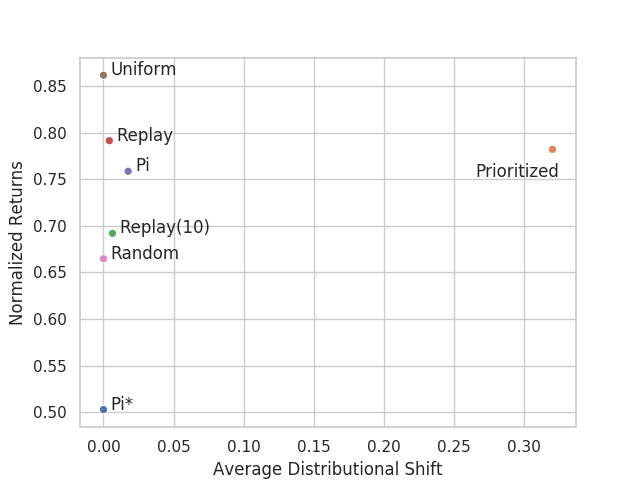
\includegraphics[width=0.99\columnwidth]{chapters/diagnosing_q/images/returns_vs_shift}
% % generated by plot_distribution_shift.py
% % data_dir = east1//2019-02-12-exact-weighting-distr-shift
% \vspace{-0.2in}
% \end{subfigure}
% ~\vline~
% \begin{subfigure}{0.3\linewidth}
% \caption{\footnotesize \label{fig:weighting_schemes} Weighting distribution versus architecture in Exact-FQI. Replay(s, a) consistently provides the highest performance. Note that Adversarial Feature Matching is comparable to Replay(s, a), but surprisingly better for small networks. }
% 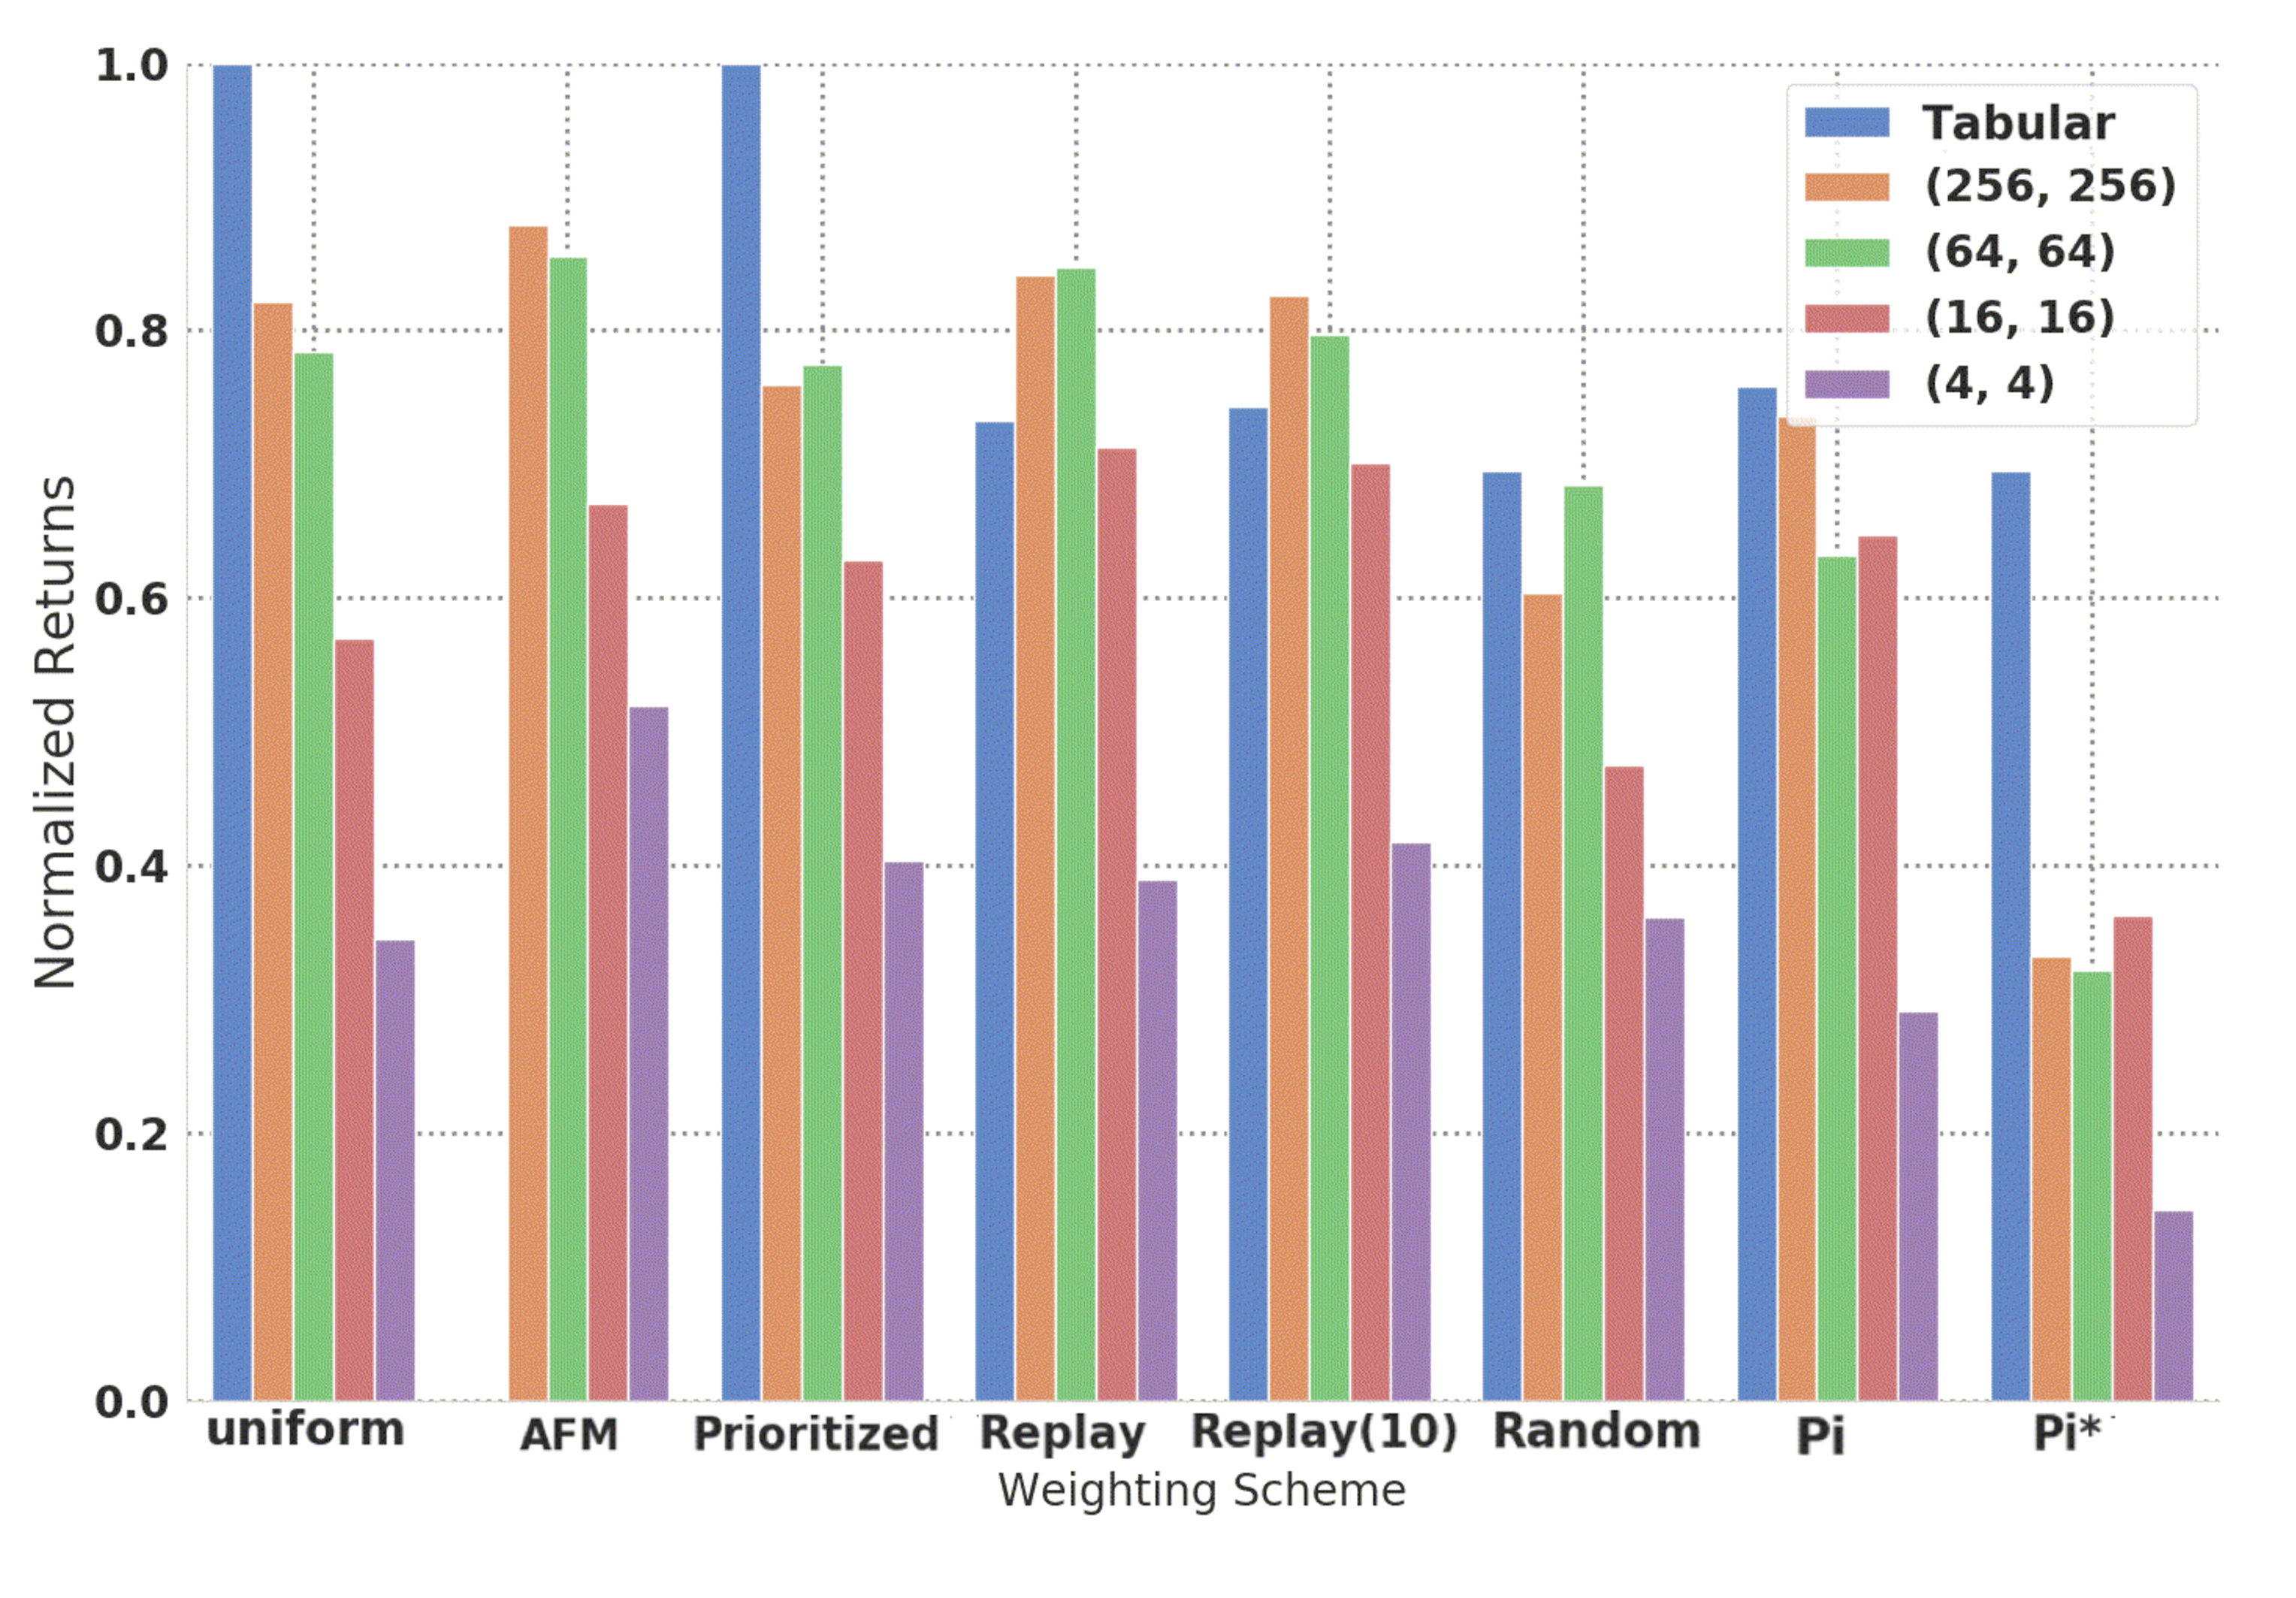
\includegraphics[width=0.99\columnwidth]{chapters/diagnosing_q/images/exact_fqi_schemes.pdf}
% % generated by plot_exact_weighting.py
% % data_dir = east1//2019-01-18-newenv-exact-weighting
% \vspace{-0.3in}
% \end{subfigure}
% ~\vline~
% \begin{subfigure}{0.3\linewidth}
% \caption{\footnotesize \label{fig:weighting_entropy_vs_returns} Normalized returns plotted against normalized entropy for different weighting distributions. All experiments use Exact-FQI with a 256x256 network. We see a general trend that high-entropy distributions lead to greater performance.}
% 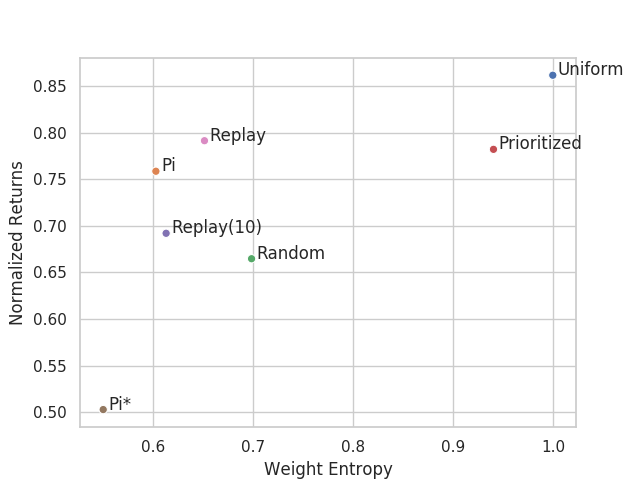
\includegraphics[width=0.99\columnwidth]{chapters/diagnosing_q/images/returns_vs_entropy}
% % generated by plot_distribution_shift.py
% % data_dir = east1//2019-02-12-exact-weighting-distr-shift
% \end{subfigure}
% \end{figure*}

\begin{wrapfigure}{r}{0.45\linewidth}
    \vspace{-0.2cm}
    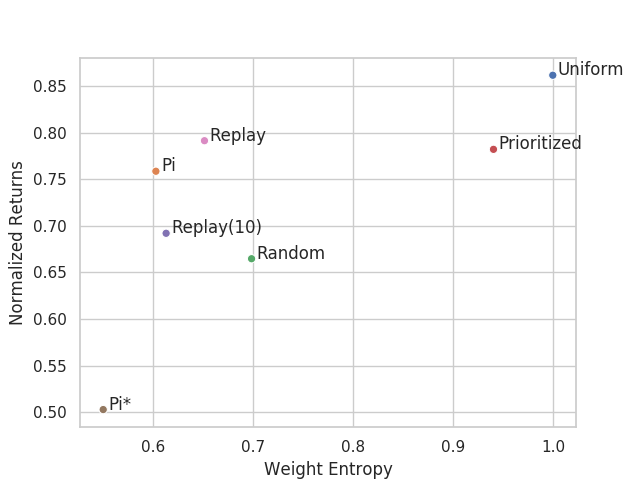
\includegraphics[width=0.99\linewidth]{chapters/diagnosing_q/images/returns_vs_entropy}
    \caption{\footnotesize \label{fig:weighting_entropy_vs_returns} Normalized returns plotted against normalized entropy for different weighting distributions. All experiments assume access to all state-action pairs with a 256x256 Q-network. We see a general trend that high-entropy distributions lead to greater performance, corroborating the uniformity hypothesis.}
    \vspace{-0.2cm}
    % generated by plot_distribution_shift.py
    % data_dir = east1//2019-02-12-exact-weighting-distr-shift
\end{wrapfigure}
We begin by studying the effect of data distributions when disentangled from sampling error. We run Q-learning with an ablation over various Q-function network architectures and data distributions and report our aggregate results in Fig.~\ref{fig:weighting_entropy_vs_returns}. $\text{Unif}(\bs, \mathbf{a})$, $\text{Replay}(\bs, \mathbf{a})$ (using a replay buffer consisting of data from a mixture of policies with different degrees of optimality), and $\text{Prioritized}(\bs, \mathbf{a})$ (weighting induced by prioritized experience replay~\citep{Schaul2016PrioritizedER}) consistently result in the highest returns across all architectures. On the other hand, relatively ``narrow'' data distributions, such as those induced the optimal policy ($\pi^*$) or only using a mixture of a few policies ($\text{Replay}(10)$) results in poor performance.
% We believe that these results are in favor of the \textit{uniformity} hypothesis: intuitively, the best distributions spread weight across larger support of the state-action space, reducing the amount of possible distributional shift. On the other hand, less-uniform distributions such as the state-action distirbution induced by the optimal policy, present multiple avenues to deviate away from the offline data distribution, resulting in larger distributional shift.
We believe that these results favor the \textit{uniformity} hypothesis: intuitively, the best distributions spread weight across a larger support of the state-action space, reducing the amount of possible distributional shift. On the other hand, less-uniform distributions, such as the state-action distribution induced by the optimal policy, present multiple avenues to deviate away from the offline data distribution, resulting in larger distributional shift.

\textbf{To summarize}, this indicates that narrow data distributions lead to worse performance compared to higher-entropy data distributions, indicating that distributional shift can have a significant impact on the performance of off-policy RL in the offline setting.
%These distributions generally result in the tightest contraction rates, and allow the Q-function to focus on high-error regions. 
%In the sampled setting, this observation motivates exploration algorithms that maximize state coverage (for example, ~\citet{hazan2018} solve an exploration objective which maximizes state-space entropy).
%However, note that in this particular experiment is distinct from exploration, as there is no sampling involved. 
%All states are observed, just with different weights, thus isolating the issue of distributions from the issue of sampling.